\documentclass[notes.tex]{subfiles}

\begin{document}

\section{Redes complexas e comunidades}

Grafos podem trivialmente ser definidos como $\G = (\V, \E)$ onde $\V$ é um conjunto dos vértices de  $\G$ e  $\E$ é um conjunto de pares não ordenados de vértices ajacentes em $\G$, i.e. as arestas.

\begin{figure}[htpb]
    \centering
    \caption{Exemplo de grafo}\label{fig:graph_example}
    \fbox{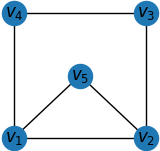
\includegraphics[width=0.4\textwidth]{figures/graph_example.png}}
    \fonte{elaborado pelo autor}
\end{figure}
\medskip

No exemplo da \autoref{fig:graph_example}, pode se representar o mesmo grafo com $\V = \{v_1, v_2, v_3, v_4, v_5\}$ e $\E = \{\{v_1, v_2\}, \{v_2, v_3\}, \{v_3, v_4\}, \{v_4, v_1\}, \{v_1, v_5\}, \{v_2, v_5\}\}$.
Dentro desse grafo, o subgrafo formato pelos vértices $v_1$, $v_2$ e $v_5$ é também um grafo completo.
A esse conjunto de vértices que forma um subgrafo completo dá-se o nome de clique \cite{fortunato2010community}.
Essa descrição de clique é utilizada como uma definição inicial do conceito de comunidade, partindo de uma perspectiva local \cite{fortunato2010community}.
Dentro desse conceito de comunidade, nomeia-se as arestas cujos dois vértices estão contidos em uma comunidade como sendo interna á comunidade.

É facilmente observável, no entanto, que essa é uma definição muito limitante de comunidade, é raro que comunidades de pessoas apresentem tanta homogeneidade a ponto de todos os membros conhecerem todos os outros membros.
De fato, \citeonline{fortunato2010community} indica que a definição precisa do que é uma comunidade varia de acordo também com o contexto de estudo, mas que algumas características são universais.
Uma comunidade, dentro de qualquer definição, deve ser um sub grafo conexo, por exemplo.

As definições são agrupadas em três classes distintas por \citeonline{fortunato2010community}:

\begin{itemize}
    \item Definição local
    \item Definição global
    \item Definição por similaridade de vértice
\end{itemize}

Essas definições não são mutuamente exclusivas, mas também não são ortogonais uma a outra.
Segundo \citeonline{fortunato2010community}, a definição local parte das características topológicas internas á comunidade.
Nominalmente, isso significa a existência de um conjunto considerável de arestas internas a comunidade e um conjunto limitado de arestas para além da comunidade.

A definição global de comunidades é aplicada aos casos onde a presença de clusters é uma característica inerente ao grafo que se está estudando \citeonline{fortunato2010community}.
Essa propriedade inerente ao grafo pode ser definida como alguma propriedade dos vértices do objeto em questão e que partindo disso se atribui pertencimento á comunidades, ou ainda por comparação com um exemplo nulo \citeonline{fortunato2010community}.
No caso de comparação com um exemplo nulo, define-se uma comunidade pela característica de uma não ser presente dentro de o que é chamado de ``grafo aleatório'' \cite{fortunato2010community}.
Essa definição de um modelo nulo é crucial para o trabalho de \citeonline{girvan2002community}, o modelo nulo considerado é um onde o grafo original é alterado de forma aos graus de todos os vértices se manterem, mas a probabilidade de dois vértices estarem ligados é constante independente de quais os vértices.

Por fim, a definição de comunidade por similaridade de vértice se baseia na tendencia de que em muitas aplicações, membros de comunidades são mais similares entre si do que seria esperado de um conjunto do mesmo tamanho escolhido aleatoriamente \cite{fortunato2010community}.
Essa definição se faz visível no trabalhos de \citeonline{akoglu2009rtg} e de \citeonline{largeron2015generating}.
Na observação desses dois trabalhos também é interessante o questionamento de como se define semelhança, \citeonline{akoglu2009rtg} representa os vértices como sequencias de caracteres de tamanhos variáveis em que a probabilidade de dois vértices estarem ligados é maior conforme mais caracteres eles compartilham; e \citeonline{largeron2015generating} representa os vértices como pontos em um espaço $n$-dimensional e define que vértices são mais semelhantes quando a distância euclideana deles é menor.

Também independente de qual definição de comunidade que se esteja utilizando, existem os conceitos de partição e cobertura.
Segundo \citeonline{fortunato2010community}, uma partição é uma divisão dos vértices de um grafo tal que cada vértice pertença a um e exatamente um cluster.
O caso de um vértice ``livre'', não pertencendo a nenhuma comunidade, é trivialmente resolvido incluindo ele á comunidade com a qual ele mais tem jacências.
Mas o caso de vértices que pertençam a mais de uma comunidade, isso é, comunidade que se sobreponham é mais interessante.
\citeonline{fortunato2010community} define uma cobertura como uma divisão dos vértices em clusters onde cada vértice pertence a um ou mais clusters.
\citeonline{fortunato2010community} também descreve o conceito de comunidades hierárquicas, como sendo comunidades cuja estrutura interna também se organiza em clusters de escala menor do que o original.

Por fim, \citeonline{fortunato2010community} oferece também o conceito de ``função de qualidade'', sendo uma função que mapeia uma partição para um espaço de comparação, usualmente em números reais, onde partições que mapeiem para valores maiores são consideradas melhores.
Segundo \citeonline{fortunato2010community} função de qualidade mais comumente utilizada é a modularidade $Q$ de \citeonline{girvan2002community}.

\begin{quadro}[htb]
\caption{\label{qua:exmp}Função modularidade $Q$}

    \begin{equasion}
    \boxed{%
        Q = \frac{1}{2m}\sum_{ij}\Bigg(A_{ij}-\frac{K_iK_j}{2m}\Bigg)\delta(C_i, C_j)
        }
    \end{equasion}

    \fonte{\citeonline{girvan2002community}}
\end{quadro}

Essa função no entanto não se aplica adequadamente ao caso de comunidades sobrepostas ou comunidades hierárquicas, para tanto, é necessário utilizar a função de modularidade estendida, conforme desenvolvido por \citeonline{shen2009detect}.

\begin{quadro}[htb]
\caption{\label{qua:exmp}Função modularidade estendida $EQ$}

    \begin{equasion}
    \boxed{%
        EQ = \frac{1}{2m}\sum_{i}\sum_{v \in C_i, w \in C_i}\frac{1}{O_vO_w}\Bigg[A_{vw} - \frac{K_iK_j}{2m} \Bigg]
        }
    \end{equasion}

    \fonte{\citeonline{shen2009detect}}
\end{quadro}

\end{document}
